\chapter{The Visual Atlas of Composition Mosaics}
\label{chap:visual-atlas}

\section*{Cartographic Conventions}

This visual catalogue displays the complete combinatorial census of all $509$ non-equivalent dihedral composition mosaics across the circular rings $\mathbb{Z}_1$ through $\mathbb{Z}_8$, ordered canonically by lattice ring order $n$, part count $s$, partition shape $\lambda \vdash n$, and intra-shape invariants.

Each drawing portrays an individual dihedral orbit through its canonical representative inscribed in a regular $n$-gon:
\begin{itemize}
    \item \textbf{Lattice Frame}: The $n$ vertices of $\mathbb{Z}_n$ are oriented with vertex $0$ at the zenith, advancing clockwise $0, 1, \dots, n-1$. A regular $n$-gon is lightly delineated in the background to establish the metric frame (for $n=1$, a circular boundary; for $n=2$, a dashed line of vertices).
    \item \textbf{Block Delineation}:
    \begin{itemize}
        \item \emph{Unigons ($d=1$)} are marked by circular nodes at the corresponding lattice vertex.
        \item \emph{Digons ($d=2$)} are drawn as prominent straight metric chords connecting the vertex pair.
        \item \emph{Inscribed Polygons ($d \ge 3$)} are drawn as shaded polygonal tiles bounded by their cyclic perimeter chords.
    \end{itemize}
    \item \textbf{Bilateral Symmetry Colouring}:
    \begin{itemize}
        \item \textbf{Blue}: Bilaterally symmetric (achiral) blocks possessing an internal axis of dihedral reflection.
        \item \textbf{Pink}: Scalene (chiral) blocks lacking reflection symmetry.
    \end{itemize}
    \item \textbf{Orbit Invariants}:
    \begin{itemize}
        \item \textbf{Upper-Left Index}: Bold global integer identifier ($1 \dots 509$) referencing the master catalogue in Section~\ref{sec:relational-datasets} and \path{data/mosaics.tsv}.
        \item \textbf{Upper-Right Ring}: Cyclic ring order $\mathbb{Z}_n$.
        \item \textbf{Lower-Right Orbit Size}: Dihedral orbit length $|\mathcal{O}| \in \{1, \dots, |D_n|\}$ under the action of $D_n$.
    \end{itemize}
\end{itemize}

\section*{Visual Plate Directory}

The 509 mosaics are distributed across ten vector plates:
\begin{itemize}
    \item \textbf{Plate 1} (Page~\pageref{plate:1}): Lattices $\mathbb{Z}_1$ through $\mathbb{Z}_5$ (Orbits 1--25).
    \item \textbf{Plate 2} (Page~\pageref{plate:2}): Lattice $\mathbb{Z}_6$ (Orbits 26--62).
    \item \textbf{Plate 3} (Page~\pageref{plate:3}): Lattice $\mathbb{Z}_7$ Part I (Orbits 63--122).
    \item \textbf{Plate 4} (Page~\pageref{plate:4}): Lattice $\mathbb{Z}_7$ Part II (Orbits 123--155).
    \item \textbf{Plates 5--10} (Pages~\pageref{plate:5}--\pageref{plate:10}): Lattice $\mathbb{Z}_8$ (Orbits 156--509).
\end{itemize}

\clearpage
\phantomsection
\label{plate:1}
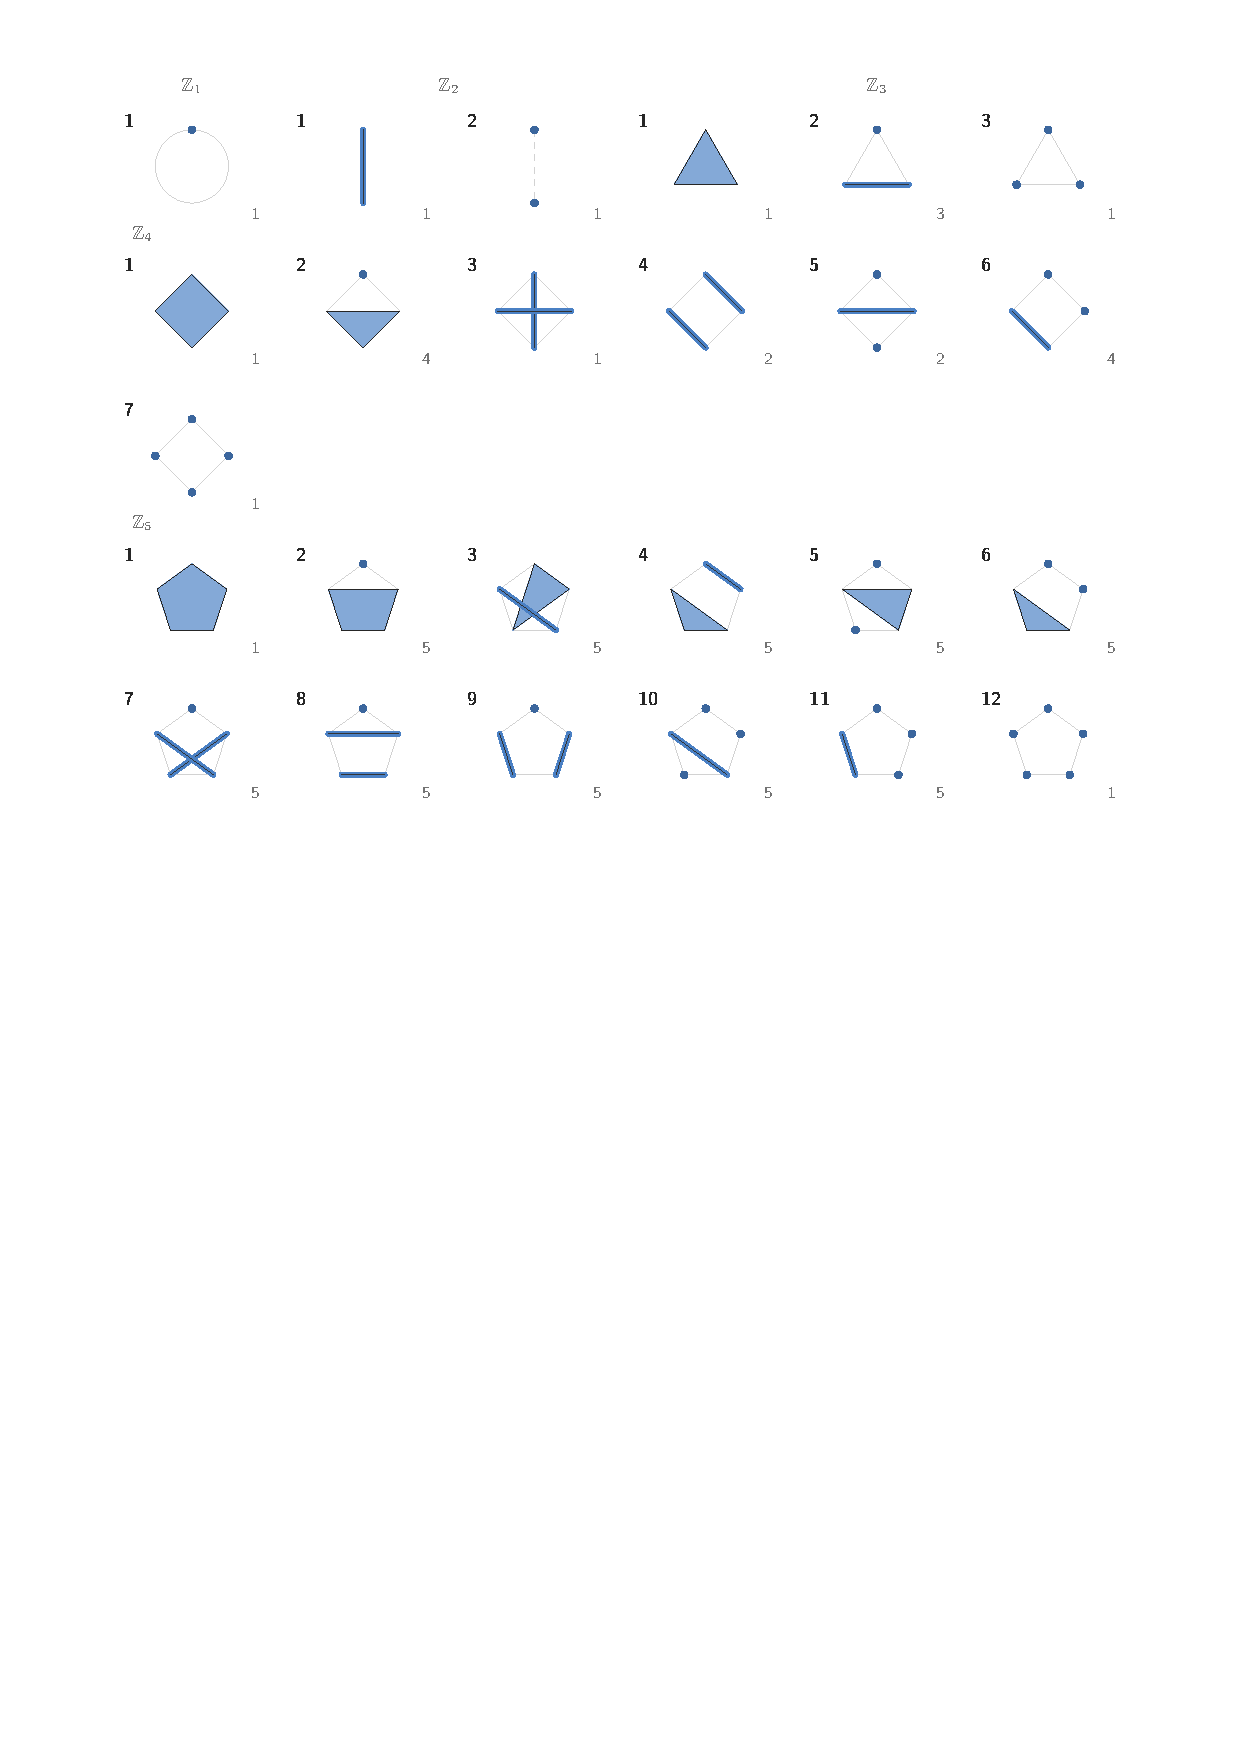
\includepdf[pages=1, offset=0 -16mm, pagecommand={\thispagestyle{headings}}]{plates/plates_z1_z8.pdf}
\phantomsection
\label{plate:2}
\includepdf[pages=2, offset=0 -16mm, pagecommand={\thispagestyle{headings}}]{plates/plates_z1_z8.pdf}
\phantomsection
\label{plate:3}
\includepdf[pages=3, offset=0 -16mm, pagecommand={\thispagestyle{headings}}]{plates/plates_z1_z8.pdf}
\phantomsection
\label{plate:4}
\includepdf[pages=4, offset=0 -16mm, pagecommand={\thispagestyle{headings}}]{plates/plates_z1_z8.pdf}
\phantomsection
\label{plate:5}
\includepdf[pages=5, offset=0 -16mm, pagecommand={\thispagestyle{headings}}]{plates/plates_z1_z8.pdf}
\phantomsection
\label{plate:6}
\includepdf[pages=6, offset=0 -16mm, pagecommand={\thispagestyle{headings}}]{plates/plates_z1_z8.pdf}
\phantomsection
\label{plate:7}
\includepdf[pages=7, offset=0 -16mm, pagecommand={\thispagestyle{headings}}]{plates/plates_z1_z8.pdf}
\phantomsection
\label{plate:8}
\includepdf[pages=8, offset=0 -16mm, pagecommand={\thispagestyle{headings}}]{plates/plates_z1_z8.pdf}
\phantomsection
\label{plate:9}
\includepdf[pages=9, offset=0 -16mm, pagecommand={\thispagestyle{headings}}]{plates/plates_z1_z8.pdf}
\phantomsection
\label{plate:10}
\includepdf[pages=10, offset=0 -16mm, pagecommand={\thispagestyle{headings}}]{plates/plates_z1_z8.pdf}
